\documentclass[12pt]{article}

% Packages
\usepackage[utf8]{inputenc}
\usepackage{amsmath}
\usepackage{amssymb}
\usepackage{graphicx}
\usepackage{hyperref}
\usepackage{amsthm}
\usepackage[margin=1in]{geometry}
\usepackage[numbers]{natbib}
\usepackage{listings}
\usepackage{algorithm}
\usepackage{algpseudocode}
\usepackage{tabularx}

% TikZ and diagram packages
\usepackage{tikz}
\usetikzlibrary{positioning,arrows,shapes,calc,decorations.pathreplacing}
\usepackage{forest}

% Theorem environments
\newtheorem{theorem}{Theorem}
\newtheorem{lemma}{Lemma}
\newtheorem{proposition}{Proposition}
\newtheorem{corollary}{Corollary}
\newtheorem{hypothesis}{Hypothesis}
\newtheorem{definition}{Definition}
\newtheorem{remark}{Remark}
\newtheorem{constraint}{Constraint}

% Title and author
\title{TranslationAI: Theory‑Driven, Ethically Engineered Machine Translation for Accessible Long‑Form Workflows}
\author{Author Name}
\date{\today}

\begin{document}
\maketitle
\begin{abstract}
This paper reconstructs and systematizes the design philosophy and technical architecture of TranslationAI, an AI‑assisted translation platform explicitly grounded in academic translation theory and software craftsmanship principles. We argue that translation quality depends less on marginal model improvements and more on the consistent application of appropriate translation strategies aligned with purpose, text type, and cultural handling requirements. TranslationAI operationalizes eight influential theoretical frameworks, integrates Hallidayan register analysis, and enforces framework‑specific rules as system‑level constraints rather than soft prompts (ref_1). A glossary‑driven memory system guarantees document‑level terminological consistency without manual maintenance. The platform couples this strategy‑first design with a rigorously engineered infrastructure: radical error transparency, multi‑layer payment verification, atomic credit accounting, abandoned‑chunk recovery, and single‑source‑of‑truth configuration. Economically, fixed per‑word pricing and very low marginal costs (down to $0.00005$ per word) reduce barriers by several orders of magnitude relative to professional human translation, in line with recent analyses of neural MT pricing and market positioning (ref_7), enabling new use cases for students, independent authors, researchers, small publishers, and cultural preservation projects. We analyze how human‑in‑the‑loop oversight is embedded at key decision points, what the system deliberately does not claim (including publication readiness and domain expertise), and how the combination of theoretical rigor, engineering reliability, and economic accessibility opens a new design space between generic machine translation and professional human work.
\end{abstract}

\section{Introduction}

Translation technologies have undergone rapid transformation over the last decade, driven by advances in neural machine translation and large language models. Mainstream systems such as generic machine translation services and conversational AI tools have made cross‑lingual access widely available, but their design remains predominantly model‑centric and algorithm‑first. They treat disparate genres and purposes with a largely uniform, opaque translation strategy, leaving users to perform strategic tailoring and quality control manually.

This paper presents TranslationAI as a contrasting design: a translation platform whose primary design axis is not model sophistication but explicit translation strategy. Its central claim is that, for long‑form, purpose‑sensitive translation, strategy matters more than raw model capability. Specifically, the system asserts that:
\begin{itemize}
  \item translation quality is determined by the systematic choice and enforcement of an appropriate theoretical framework;
  \item users must be given transparent control over purpose, communicative approach, and cultural positioning;
  \item reliability, honesty, and consistency are as important as raw accuracy; and
  \item economic accessibility at scale requires a radically different cost structure than professional human translation (ref_7).
\end{itemize}

We synthesize the platform's guiding philosophy, the translation‑theoretical foundations it implements, and the engineering patterns that support its reliability and transparency. The result is a conceptual and technical blueprint for theory‑driven AI translation that deliberately positions itself between generic automated systems and fully human professional workflows.

The discussion proceeds as follows. We first articulate the core insight that motivates the system and describe the missing layer between raw AI capability and high‑quality translation. We then formalize the translation‑theory foundation, focusing on eight implemented frameworks and their operationalization as strict constraints. Subsequent sections analyze the limitations of existing solutions, the alternative architectural choices TranslationAI makes, the controls and affordances provided to users, and the system's craftsmanship: glossary‑driven memory, payment ethics, security mechanisms, and operational robustness. We then examine the real benefits delivered to users, the scope limitations the system explicitly acknowledges, the human‑in‑the‑loop design, and the economic implications of orders‑of‑magnitude price reduction (ref_7). We conclude by situating TranslationAI as an instance of computational translation theory in practice and outlining the broader research and design questions it raises.

\section{Core Philosophy and Systemic Honesty}

The foundational insight behind TranslationAI is that translation quality is not primarily a function of which model is used, but of how that model is constrained and directed by an explicit, coherent translation strategy. A children's picture book, a doctoral thesis, a commercial novel, and a safety‑critical technical manual call for fundamentally different balances of fidelity, readability, and cultural adaptation. Yet most automated systems treat all four as instances of the same generic task: \emph{translate this text}.

TranslationAI treats this homogenization as a design error. It posits an intermediate "missing layer" between raw AI capability and user‑visible output: translation theory expertise embodied as machine‑enforceable rules. The system embeds the decision logics developed in translation studies into its architecture, so that users configure strategies in terms of purpose and cultural positioning instead of crafting ad hoc prompts or relying on opaque defaults. In this sense, the platform is not merely \emph{using} AI to translate; it is using AI to \emph{execute} pre‑specified translational programs.

A second pillar of the philosophy is radical honesty. The system rejects silent fallbacks, implicit defaults that alter billing or quality, and quiet omission of failed units of work. This commitment manifests in a general design invariant:
\begin{equation*}
  \text{If a critical operation fails, the system must either succeed atomically or fail visibly with an explicit error.}
\end{equation*}

This invariant governs payment processing (multi‑layer verification, no silent acceptance on partial signals), credit deductions (atomic transactions with audit trails), translation chunking (explicit pending/processing/completed/failed states with visible failure), and configuration validation (errors on invalid quality tiers rather than hidden downgrades). The ethical premise is that trust arises from precise, observable failure modes rather than from opaque resilience.

These two commitments—strategy‑first translation and error transparency—frame every subsequent architectural choice. The platform's design can thus be read as an extended attempt to operationalize both commitments rigorously in an AI‑augmented translation workflow.

\section{Translation Theory as Operational Foundation}

Translation studies has produced a rich ecology of theoretical frameworks intended not as purely abstract constructs but as practical decision systems for working translators. TranslationAI adopts eight such frameworks as first‑class architectural components and couples them with Hallidayan register analysis as an upstream analytic stage (ref_1).

\subsection*{Register Analysis as Input Typology}

Before selecting a translation strategy, the system performs a register analysis of the source text along three dimensions derived from systemic functional linguistics:
\begin{itemize}
  \item \emph{Field}: subject matter and degree of technical specialization;
  \item \emph{Tenor}: social relation between author and reader, including formality and power distance; and
  \item \emph{Mode}: medium and rhetorical organization (e.g., written exposition versus dialogic interaction).
\end{itemize}

Following Halliday's foundational account of grammatical categories and their relation to context (ref_1), the system treats these variables as determinants of expected lexico‑grammatical patterns rather than as mere labels. From this analysis it derives metadata such as the domain (e.g., medical, literary, legal), formality, and structural mode. These metadata serve three purposes: (i) recommending an appropriate framework (e.g., semantic translation for highly formal academic material), (ii) pre‑selecting plausible purposes on the frontend (e.g., academic versus entertainment), and (iii) avoiding redundant re‑analysis by storing results for reuse. Crucially, these register features are \emph{not} injected directly into translation prompts; instead, frameworks define their own stylistic regimes to prevent theoretical conflict.

\subsection*{Eight Implemented Frameworks}

The platform implements eight influential frameworks as configurable strategies. Each framework is encoded as a structured set of mandatory rules and explicit prohibitions, enforced at the system level.

\paragraph{Skopos Theory.} Skopos Theory foregrounds translation purpose as the primary determinant of all translational decisions. Operationally, TranslationAI asks users to specify purposes such as entertainment, learning, literary appreciation, or academic study. The selected purpose then activates a rule set asserting the supremacy of that purpose over other considerations. For example, an entertainment skopos may permit substantial adaptation for readability, whereas an academic skopos demands preservation of structural and cultural features even at the cost of fluency.

\paragraph{Register Theory.} Register Theory is used primarily at the analysis stage, not as a direct translation regime. By categorizing text in terms of field, tenor, and mode, the system can algorithmically infer whether source‑oriented or target‑oriented strategies are appropriate, and whether specialized terminology handling is required. This inference, grounded in systemic functional accounts of how contextual variables shape discourse (ref_1), then informs framework recommendations and auto‑configuration.

\paragraph{Semantic Translation.} Newmark's semantic translation prioritizes source‑text form and meaning, preserving syntactic structure, ambiguity, and connotation. In TranslationAI, selecting this framework triggers dozens of explicit constraints such as: maintain sentence structure where linguistically possible, preserve ambiguities, prohibit idiom adaptation, forbid restructuring solely for fluency, and disallow cultural substitution except via tightly scoped notes. The cumulative effect is a systematically source‑oriented output suitable for academic, legal, and technical contexts.

\paragraph{Communicative Translation.} In contrast, communicative translation aims to reproduce contextual meaning in natural target‑language form. The rules now invert: restructure freely for fluency, adapt idioms to target equivalents, replace unfamiliar cultural references when necessary for comprehension, and privilege reader experience over formal mirroring. This framework is recommended for fiction, marketing, and general‑audience texts where immersion outweighs literalism.

\paragraph{Foreignization.} Venuti's foreignization strategy preserves the visible "otherness" of source culture, explicitly resisting the ethnocentric fluency that erases difference (ref_2). System rules enforce the retention of foreign proper names, maintenance of culturally specific practices, allowance of stylistic strangeness, and explicit prohibition of naturalizing transformations. The translation is intentionally marked as a translation, supporting cultural authenticity and distance.

\paragraph{Domestication.} Domestication, by contrast, systematically adapts source materials to target‑culture norms, corresponding to the domesticating practices Venuti critiques as dominant in many publishing contexts (ref_2). Rules encourage replacing culture‑bound references with functional local analogues, naturalizing names when appropriate, and eliminating "translation feel". This is especially suitable for commercial fiction, children's literature, and mass‑market content seeking maximal accessibility.

\paragraph{Functionalist Model.} Nord's functionalist model introduces an explicit ethical dimension by balancing functional adequacy with loyalty to the source. TranslationAI encodes this as a decision schema applied at the micro‑decision level: for each choice, evaluate (i) whether it serves the skopos and (ii) whether it maintains loyalty; accept only those satisfying both, and otherwise seek a compromise rather than absolute priority of one dimension.

\paragraph{Five Equivalences.} Koller's five equivalence types—denotative, connotative, text‑normative, pragmatic, and formal‑aesthetic—are implemented as a multi‑dimensional quality checklist (ref_3). Empirical work on multidimensional assessment of translation quality demonstrates that evaluating translations along multiple equivalence axes captures nuances that single‑score metrics miss, especially in literary and stylistically marked texts (ref_3). For high‑tier translations, the system instructs the AI to evaluate output against all five criteria, and when conflicts arise, to prioritize those equivalence types aligned with the primary function of the text, documenting trade‑offs in translation notes.

\subsection*{From Theory to Constraint}

Across all frameworks, TranslationAI's central move is to treat theoretical guidance as \emph{constraints}, not hints. System prompts encode mandatory requirements ("you must"), explicit prohibitions ("forbidden"), and priority hierarchies. The AI is not invited to approximate a style but tasked with executing a defined strategy. If required instructions cannot be followed, the correct behavior is to fail with an error, not to silently deviate. This turns translation theories into programmable regimes that can be applied consistently across tens of thousands of words and evaluated using multidimensional quality criteria inspired by contemporary translation quality research (ref_3).

\section{Limitations of Existing Translation Approaches}

\subsection*{Qualitative Comparison of Translation Paradigms}
A LaTeX table summarizing qualitative differences between generic machine translation, general-purpose AI tools, professional human translation, and the TranslationAI approach.

\begin{tabular}{|l|c|c|c|c|}
\hline
Aspect & Machine MT & General AI Tools & Human Translators & TranslationAI \\
\hline
Strategy explicitness & Low & Medium & High & High \\
User control over theory & None & Prompt-based & Indirect & Direct \\
Document-level consistency & Low & Low--Medium & High & High \\
Cost per word & Very low & Variable & High & Very low \\
Turnaround time & Seconds & Seconds--Minutes & Weeks--Months & Hours--Days \\
Cultural configurability & None & Limited & High & High \\
Need for human review & High & High & Medium & Medium--High \\
Accessibility for individuals & High & Medium & Low & High \\
\hline
\end{tabular}

The design of TranslationAI is explicitly reactive to perceived structural limitations in three prevailing translation paradigms: generic machine translation services, general‑purpose conversational AI tools, and professional human translation.

\subsection*{Generic Machine Translation}

Mainstream machine translation systems operate essentially as one‑size‑fits‑all solutions (ref_4). A travel guide, a legal contract, a poem, and a marketing brochure are processed via the same internal model with little to no exposure of strategy to users. Survey work on controllable neural machine translation documents how most deployed systems still offer only coarse control over style or register, with limited support for systematically aligning translations with user‑specified communicative goals (ref_4). Three systemic issues follow.

First, \emph{strategy opacity}: users cannot specify whether cultural references should be preserved or adapted, whether syntactic structure should be mirrored or reconfigured, or what skopos the translation should serve. Outcomes reflect statistical patterns in training data, not the user's purpose.

Second, \emph{sentence‑level independence}: many systems handle sentences or small segments quasi‑independently, producing document‑level inconsistency in names, terminology, and stylistic choices. The same proper name may appear in multiple transliterations; the same technical term may receive inconsistent renderings across a long document.

Third, \emph{no project‑level control}: there is little support for glossary enforcement, chunk‑level progress tracking, or failure visibility. Users cannot easily see which parts of a long document failed or were skipped, nor can they enforce terminology across the document.

\subsection*{General‑Purpose AI Tools}

Conversational models can be instructed to translate and accept complex prompts. This adds flexibility but shifts the burden of expertise to users.

Users must articulate translation strategies in prompt form, which presupposes knowledge of translation theory and the ability to translate that theory into precise instructions. Vague prompts such as "make it natural" or "keep it accurate" under‑specify crucial trade‑offs. Inconsistent prompting across chunks leads to drift in terminology and style.

Context window limits necessitate chunking for long documents (ref_5). Analyses of large language models emphasize that, despite steadily increasing context lengths, practical capacity remains bounded, and long inputs must still be segmented for efficient processing (ref_5). Absent explicit memory structures, each chunk is treated largely in isolation. Names and terms may vary. There is typically no built‑in project management: no automatic glossary, no systemic reinjection of prior decisions into later chunks, no standardized abandonment recovery, and no billing tied to per‑word predictability.

\subsection*{Professional Human Translation}

Professional human translators remain the gold standard for publication‑ready work, especially in domains requiring deep cultural or technical expertise. However, this model creates a substantial accessibility gap.

Costs per word are high relative to the budgets of students, independent authors, and small organizations. Market studies of NMT pricing and human translation services show persistent per‑word price differentials, with professional human work commanding substantially higher rates even when aided by MT (ref_7). Turnaround times for long documents are measured in weeks or months. Availability is constrained by language pair and specialization. These constraints make exploratory, experimental, or high‑volume translation economically and logistically infeasible for many potential users.

TranslationAI does not seek to displace professional translation where certification, liability, and artistic excellence are required. Instead, it targets the substantial space of projects where human translation is either unaffordable or unavailable, and where strategic, theory‑driven AI output can provide high‑quality drafts or final translations for low‑risk uses.

\section{A Strategy‑First Architecture for AI Translation}

\subsection*{End-to-End Strategy-First Translation Pipeline}
A high-level TikZ diagram illustrating the main stages of the TranslationAI pipeline: register analysis, strategy selection, glossary extraction and translation, chunked translation with glossary enforcement, and human review.

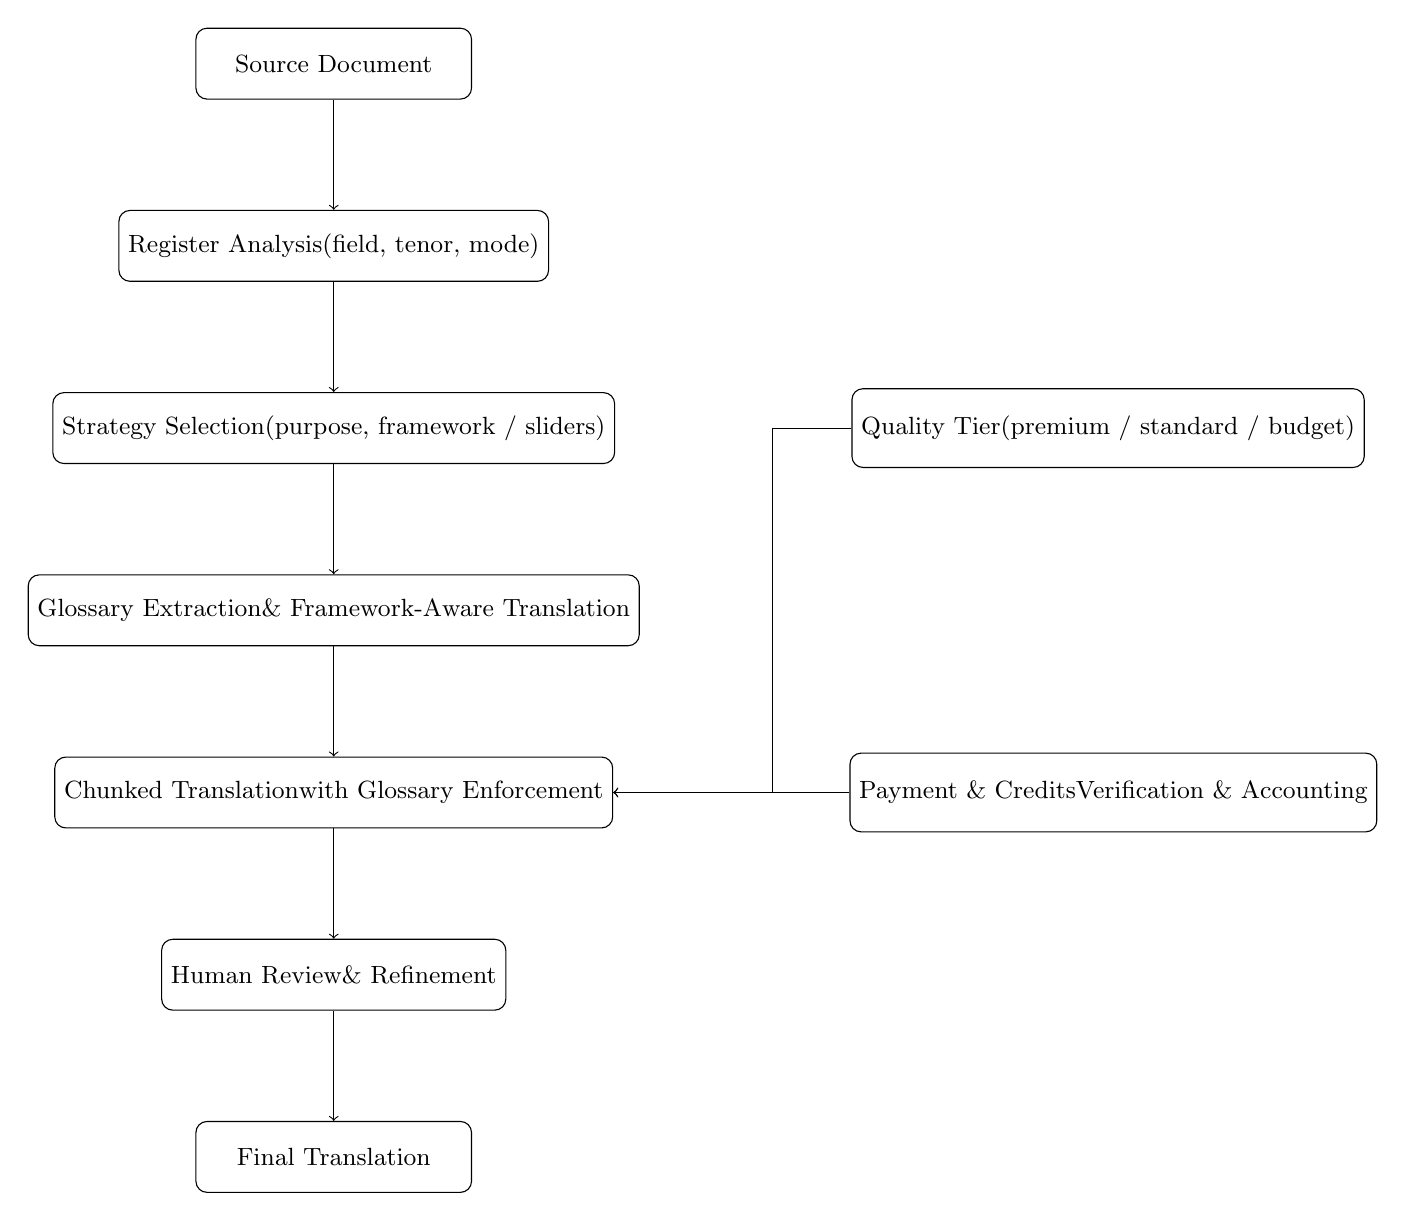
\begin{tikzpicture}[font=\small, node distance=1.4cm]
  % Nodes
  \node[draw, rectangle, rounded corners, minimum width=3.5cm, minimum height=0.9cm] (source) {Source Document};
  \node[draw, rectangle, rounded corners, below=of source, minimum width=3.5cm, minimum height=0.9cm] (analysis) {Register Analysis\\(field, tenor, mode)};
  \node[draw, rectangle, rounded corners, below=of analysis, minimum width=4.2cm, minimum height=0.9cm] (strategy) {Strategy Selection\\(purpose, framework / sliders)};
  \node[draw, rectangle, rounded corners, below=of strategy, minimum width=4.8cm, minimum height=0.9cm] (glossary) {Glossary Extraction\\\& Framework-Aware Translation};
  \node[draw, rectangle, rounded corners, below=of glossary, minimum width=4.5cm, minimum height=0.9cm] (chunks) {Chunked Translation\\with Glossary Enforcement};
  \node[draw, rectangle, rounded corners, below=of chunks, minimum width=3.8cm, minimum height=0.9cm] (human) {Human Review\\\& Refinement};
  \node[draw, rectangle, rounded corners, below=of human, minimum width=3.5cm, minimum height=0.9cm] (final) {Final Translation};

  % Arrows
  \draw[->] (source) -- (analysis);
  \draw[->] (analysis) -- (strategy);
  \draw[->] (strategy) -- (glossary);
  \draw[->] (glossary) -- (chunks);
  \draw[->] (chunks) -- (human);
  \draw[->] (human) -- (final);

  % Side node for quality tiers
  \node[draw, rectangle, rounded corners, right=3.0cm of strategy, minimum width=3.0cm, minimum height=1.0cm] (quality) {Quality Tier\\(premium / standard / budget)};
  \draw[->] (quality.west) -- ++(-1.0,0) |- (chunks.east);

  % Side node for payment and credits
  \node[draw, rectangle, rounded corners, right=3.0cm of chunks, minimum width=3.2cm, minimum height=1.0cm] (payment) {Payment \& Credits\\Verification \& Accounting};
  \draw[->] (payment.west) -- ++(-1.0,0) |- (chunks.east);
\end{tikzpicture}

TranslationAI's architecture is built to treat the AI model as a strategy executor operating within a larger, theory‑driven pipeline. Four architectural principles are central: explicit strategy selection, glossary‑backed consistency, intelligent phase control, and transparent configuration.

\subsection*{Strategy Selection Before Translation}

Rather than immediately invoking a translation model, the system requires users to answer a sequence of strategic questions: What is the primary purpose of the translation? Who is the intended audience? How should cultural elements be handled? Is the text primarily academic, literary, entertainment, or educational?

These inputs combine with register analysis to select or configure a translation framework. The system can operate in two mutually exclusive modes:
\begin{itemize}
  \item \emph{Framework mode}: users directly choose one of the eight implemented theories, accepting its full rule set.
  \item \emph{Manual mode}: users adjust two continuous sliders: an approach axis from semantic to communicative, and a cultural axis from foreignization to domestication. From these scalar positions, the system synthesizes a custom rule set for the AI.
\end{itemize}

The mutual exclusivity avoids contradictory instruction sets (for example, selecting semantic translation while placing the approach slider at the extreme communicative end).

\subsection*{Consistency Through Glossary Memory}

Professional translators rely on translation memories and glossaries to maintain terminological consistency. TranslationAI replicates this capability automatically through an AI‑powered glossary system.

After initial analysis, the system performs a book‑level scan to extract 50–200 key terms, prioritizing frequency, semantic importance, and type (characters, places, cultural concepts, technical terminology, organizations, significant objects). Each term is categorized and then translated once in a manner consistent with the chosen framework and cultural settings. For example, a personal name may be left in original form under foreignization but adapted under domestication.

During chunk translation, the glossary is injected as a set of mandatory constraints: each listed source term \emph{must} be rendered exactly as specified wherever it appears. The model is explicitly forbidden from introducing variation. This mechanism guarantees document‑level consistency without manual spreadsheet management.

\subsection*{Intelligent Phase Control}

Long‑form translation is decomposed into phases:
\begin{enumerate}
  \item Register‑based analysis of the entire text;
  \item glossary term extraction;
  \item glossary translation according to current configuration; and
  \item chunked translation with glossary context.
\end{enumerate}

To avoid redundant computation and billing, the system selectively reruns only those phases whose outputs are invalidated by configuration changes. Analysis and term extraction are cached in persistent storage; on subsequent runs, these phases are skipped unless the text or relevant metadata change. Glossary translation is always rerun when strategy settings change, since term renderings are framework‑dependent. Chunk translation is always fresh for each configuration.

This selective recomputation achieves a balance between efficiency and correctness: expensive global analyses are not needlessly repeated, but translated content always reflects the current strategic configuration.

\subsection*{Transparent Control and Costing}

The system exposes all major strategic and economic parameters to users. They see:
\begin{itemize}
  \item the detected register profile and its implications for framework recommendations;
  \item available frameworks and their priorities and prohibitions;
  \item the exact AI model to be used in each quality tier;
  \item per‑word pricing by tier; and
  \item an exact cost estimate for a given document, computed deterministically from word count, consistent with observed linear per‑word pricing models in contemporary MT markets (ref_7).
\end{itemize}

This contrasts with token‑based systems whose costs are difficult to predict ex ante. Fixed per‑word pricing enables concrete budgeting for individuals and organizations, and supports experimentation across strategies without risk of large, unpredictable charges.

\section{User Control, Quality Tiers, and Informed Choice}

\subsection*{Cost Function for Deterministic Per-Word Pricing}
A simple equation capturing how TranslationAI computes exact project costs as a function of word count and quality tier.

\begin{equation}
  C(w, q) = w \cdot p(q),
\end{equation}
where $C(w, q)$ is the total cost of a translation project, $w$ is the word count of the source document, and $p(q)$ is the fixed per-word price associated with the selected quality tier $q$ (e.g., budget, standard, premium).

User empowerment in TranslationAI operates along three axes: strategic control, quality–budget control, and information for decision‑making.

\subsection*{Strategic Control via Purpose and Sliders}

Purpose selection provides a high‑level alignment between the translation and user goals: entertainment, learning, literary, or academic. Each purpose presets or biases internal strategy choices: for example, entertainment purpose licenses freer adaptation and fluency, whereas academic purpose constrains the system toward source fidelity.

Beyond purpose, users operate either in framework mode (selecting a named theory) or in manual mode using two sliders:
\begin{itemize}
  \item \emph{Approach slider} (0–100): 0 approximates a fully semantic stance (source‑structure preservation), 100 approximates a fully communicative stance (target‑fluency priority), and intermediate values encode graded compromises.
  \item \emph{Cultural slider} (0–100): 0 approximates complete foreignization, 100 complete domestication, with intermediate values representing partial adaptation.
\end{itemize}

From these scalar inputs, the system generates parameterized instruction sets. Thus, non‑experts can configure complex translational behavior through intuitive controls, without naming or understanding formal theories.

\subsection*{Quality Tiers and Cost Alignment}

Three quality tiers expose a controlled trade‑off between model capability and cost:
\begin{itemize}
  \item \emph{Premium}: highest‑capacity models with large context windows, at approximately $0.00025$ per word; suitable for high‑stakes literary or professional drafts.
  \item \emph{Standard}: balanced models with strong performance at approximately $0.0001$ per word; suitable for most general purposes.
  \item \emph{Budget}: economical models at approximately $0.00005$ per word; suitable for drafts, comprehension, and high‑volume experimentation.
\end{itemize}

The pricing function can be represented schematically as
\begin{equation*}
  C(w, q) = w \cdot p(q),
\end{equation*}
where $w$ is the word count and $p(q)$ is the per‑word price associated with quality tier $q$. Because $p(q)$ is fixed, $C$ is exactly predictable before processing and conforms to the linear per‑word pricing structures observed in empirical studies of MT and human translation markets (ref_7).

Users can thus match quality to use case: premium for near‑publication drafts, standard for everyday translation, budget for exploratory or pedagogical tasks.

\subsection*{Informed Decision‑Making}

Before execution, users are presented with a consolidated configuration summary: detected register features and their implications, chosen purpose, selected framework or slider positions, quality tier, model, word count, and precise cost. Explanatory text clarifies what each framework entails and what each slider position means in practice.

The underlying rationale is that translation configuration is not a mere technical detail but a normative choice about how to treat a text. Providing intelligible rationales allows users to make reflective, not accidental, commitments about fidelity, adaptation, and reader experience.

\section{Software Craftsmanship and System Reliability}

Beyond its theoretical foundations, TranslationAI embodies a set of software engineering practices aimed at reliability, maintainability, and ethical handling of money and data.

\subsection*{Theory as Architecture}

Frameworks are implemented as shared modules, not copy‑pasted prompt templates. A single source of truth for each theory's rules resides in a dedicated module; all translation functions import from this module. Similarly, models, pricing, and supported languages are defined once in centralized configuration artifacts.

This single‑source‑of‑truth design eliminates drift: when a framework rule is corrected or refined, the change automatically propagates to all workflows. Pricing updates occur in a single configuration table, instantly affecting cost estimates and billing logic coherently. Language additions or corrections are made exactly once.

\subsection*{Glossary System as Automated Translation Memory}

The glossary mechanism functions as a translation memory without manual upkeep. AI handles extraction and classification; the system handles enforcement. This division of labor recognizes that:
\begin{itemize}
  \item humans are better at defining high‑level strategies and reviewing complex edge cases; and
  \item machines are better at exhaustive pattern detection, consistency enforcement, and large‑scale repetition.
\end{itemize}

By converting the glossary into hard constraints at translation time, the system guarantees that key nomenclature remains stable regardless of chunking or internal model variability.

\subsection*{Payment Integrity and Atomic Credits}

Payment verification employs five independent checks: confirmation with the payment provider's API, project existence and state validation, user ownership confirmation, session identifier matching, and amount consistency between expected and received payments. Only when all checks succeed is a project marked as paid.

Credit operations are implemented as atomic transactions under row locking. A typical deduction operation can be modeled as:
\begin{enumerate}
  \item lock user's credit record;
  \item read current balance $B$;
  \item if $B < C$ (required credits), abort with error;
  \item else set balance to $B - C$ and insert a transaction record;
  \item commit or roll back the entire operation as a unit.
\end{enumerate}

This design precludes race conditions and partial states, which is especially important when multiple translations are initiated in parallel from the same account.

\subsection*{Abandoned Chunk Recovery}

Long‑running translation jobs may encounter transient failures: timeouts, network outages, or process crashes. To prevent indefinite stalling, the system monitors chunks stuck in a processing state beyond a fixed threshold (e.g., five minutes) and automatically resets their status to pending, making them eligible for reprocessing.

This repeating recovery cycle continues until chunks either succeed or accumulate enough failures to justify explicit user notification. The process is transparent to users, who see eventual completion rather than hung jobs that require manual intervention.

\subsection*{Single Source of Truth and Maintainability}

The insistence on central configuration for pricing, models, languages, and frameworks is a deliberate response to the typical entropy of large systems. By ensuring that no critical parameter is defined in more than one place, the platform reduces the risk of contradictory behavior and simplifies maintenance. This architectural discipline is invisible to end users but central to long‑term reliability.

\section{User Benefits and Practical Outcomes}

The combination of theoretical rigor and engineering discipline yields a set of concrete benefits for diverse user groups. These benefits can be grouped under strategic access, consistency, economic accessibility, speed, and suitability for human refinement.

\subsection*{Expert‑Level Strategy Without Formal Training}

By embedding translation frameworks as selectable strategies, the system allows non‑experts to harness decades of scholarly and professional reflection. A student, author, or researcher need only understand questions such as "Should I preserve cultural elements or adapt them?" rather than mastering the terminology of foreignization or Skopos Theory. The platform operationalizes those answers in precise rules, including explicit choices between foreignizing and domesticating approaches as characterized by Venuti (ref_2).

\subsection*{Consistency at Scale}

Automated glossary extraction and enforcement produce professional‑grade terminological consistency across tens of thousands of words. This eliminates a class of errors—drifting character names, inconsistent technical terms—that are particularly jarring in long‑form content and tedious to correct by hand.

\subsection*{Transparent and Predictable Costs}

Fixed per‑word pricing and visible estimates prior to processing allow users to budget accurately. An independent author can compute the cost of translating a series of novels; a student can calculate the cost of translating a corpus of research articles. Promo credits and subscription word quotas map straightforwardly onto expected project sizes, mirroring the predictable per‑unit pricing structures documented in recent studies of NMT and human translation markets (ref_7).

\subsection*{Cultural Handling Aligned with Intent}

Explicit configuration of cultural positioning ensures that the treatment of culture‑bound elements matches user intent: foreignization for cultural study and authenticity, domestication for commercial accessibility, or graded intermediate approaches. This avoids the unexamined cultural defaults embedded in many generic systems and aligns with debates on the ethical and political stakes of domestication and foreignization (ref_2).

\subsection*{Speed and Parallelism}

Compared with human translation, the platform reduces typical turnaround times for book‑length documents from weeks or months to hours. Research on machine translation‑enhanced workflows shows substantial productivity gains for professional users, with MT drafts significantly shortening overall translation time (ref_6). By automating analysis, glossary construction, and consistent drafting, TranslationAI extends such gains to non‑professional users and high‑volume scenarios.

\subsection*{High‑Quality Drafts for Human‑in‑the‑Loop Workflows}

The system targets output quality in the range where human editors can focus on nuance, creativity, and domain‑specific corrections rather than wholesale rewriting. Professional translators can use TranslationAI as a drafting tool that reduces manual workload while retaining final editorial control (ref_6). Non‑professionals can use it to obtain usable translations for low‑risk or internal purposes, with the option of additional human refinement when stakes warrant.

\section{Explicit Non‑Goals and Limitations}

TranslationAI articulates several boundaries on its own capabilities. These constraints are both ethical disclosures and design choices.

\subsection*{No Claim to Publication‑Ready Perfection}

The system does not present its output as fully publication‑ready without review. Factors such as textual complexity, language pair, and technical domain introduce variability in quality. The expectation is that serious publications—especially literary, legal, and technical—will involve human review and refinement, using AI output as an accelerated draft rather than an endpoint.

\subsection*{Not a Real‑Time System}

TranslationAI is designed for batch processing of long‑form documents, not for real‑time conversational translation or live subtitling. Its architecture—full‑text analysis, glossary extraction, and chunked processing under a chosen framework—is optimized for whole‑document coherence rather than low‑latency interaction.

\subsection*{No Substitute for Deep Domain Expertise}

While contemporary AI models have broad general knowledge, they do not reliably substitute for specialized expertise in medicine, law, advanced science, or engineering. For high‑risk or high‑liability content, domain experts or specialized translators remain necessary to ensure terminological precision and conceptual correctness.

\subsection*{No Claim to Creative Brilliance}

The system does not aim to replicate the creative feats of exceptional human literary translators who sometimes produce target texts that are works of art in their own right. AI can adhere to strategies and maintain consistency, but inventing culturally situated metaphors, reconstructing intricate wordplay, or achieving poetic resonance across languages remains predominantly a human creative task.

\section{Human-in-the-Loop Design and Oversight}

\subsection*{Human–AI Collaboration as Functional Composition}
A short LaTeX display expressing the conceptual model of how human configuration, AI execution, and human refinement compose into a final translation.

\begin{equation}
  T_{\text{final}} = H\bigl(T(\text{Source} \mid S, M)\bigr),
\end{equation}
where $S$ denotes the human-chosen strategy (purpose, framework or sliders), $M$ denotes system-constructed metadata and memory (register profile, glossary), $T$ is the AI translation operator constrained by $S$ and $M$, and $H$ is the human refinement operator applied post-translation.

Rather than automating translation end‑to‑end, TranslationAI embeds human judgment at critical junctures while delegating repetitive and large‑scale tasks to AI.

\subsection*{Stages of Human Oversight}

The workflow includes multiple review stages:
\begin{enumerate}
  \item \emph{Post‑analysis review}: users inspect register analysis, extracted metadata (e.g., genre, domain), and framework recommendations, correcting misclassifications or overriding choices.
  \item \emph{Strategy configuration}: users select purpose, frameworks or slider positions, and quality tiers, making explicit normative decisions about fidelity and adaptation.
  \item \emph{Configuration confirmation}: before processing, users review a consolidated summary to catch misconfigurations (e.g., wrong target language or tier).
  \item \emph{Glossary review} (planned): users may adjust AI‑proposed term translations and add missing key terms before they are enforced.
  \item \emph{Post‑translation editing}: users revise the output for nuance, stylistic refinement, domain‑specific accuracy, and creative quality.
\end{enumerate}

This structure embodies a division of labor principle: AI performs tasks characterized by volume, repetition, and rule‑following; humans handle strategy selection, exception handling, ethical judgments, and creative improvement.

\subsection*{Conceptual Model of Collaboration}

The human–AI collaboration can be conceptualized as a composition of functions. Let $S$ denote strategic configuration chosen by the human, $M$ the analysis and memory structures constructed by the system (register profile, glossary), and $T$ the translation function executed by the AI under $S$ and $M$. The human editor then applies a refinement function $H$ to the AI's output:
\begin{equation*}
  \text{Final Translation} = H\bigl(T(\text{Source} \mid S, M)\bigr).
\end{equation*}

Here $H$ is not an optional afterthought but an integral part of workflows where stakes justify additional human investment. This aligns with empirical findings that MT‑enhanced workflows are most effective when professional translators remain in the loop as revisers and decision‑makers rather than passive post‑editors (ref_6).

\section{Economic Accessibility and Its Implications}

A defining property of TranslationAI is its pricing structure, which reduces per‑word costs by several orders of magnitude relative to standard professional rates. This has both direct and systemic implications.

\subsection*{Magnitude of Price Reduction}

If $p_{\text{human}}$ denotes typical professional rates and $p_{\text{AI}}$ denotes TranslationAI rates, then for many scenarios
\begin{equation*}
  \frac{p_{\text{human}}}{p_{\text{AI}}} \in [400, 6000] \quad \text{(ref\_7)}.
\end{equation*}

This range reflects recent analyses of how neural machine translation has been positioned in the market, with human providers maintaining substantially higher per‑word prices even when integrating MT into their workflows (ref_7). For a 60{,}000‑word text, this transforms a cost scale from thousands or tens of thousands of dollars to single‑ or low double‑digit amounts. Projects that were previously inconceivable—such as translating entire backlists, large research corpora, or numerous experimental variants—become tractable.

\subsection*{Beneficiary Groups}

Multiple communities stand to benefit:
\begin{itemize}
  \item \emph{Independent authors}, who can test multiple language markets before committing to professional translation.
  \item \emph{Students and researchers}, who can translate many research articles or primary sources within minimal budgets.
  \item \emph{Small publishers}, who can perform low‑cost exploratory translations of catalogues.
  \item \emph{Educational institutions}, which can make teaching materials and scholarship accessible in multiple languages.
  \item \emph{Cultural and preservation projects}, which can translate large archives or oral histories that lack commercial potential.
\end{itemize}

\subsection*{Newly Possible Workflows}

Low marginal costs and predictable pricing enable new practices: parallel translation into many languages for market testing; volume translation of large, previously neglected corpora; iterative retranslation under varying strategies to study comparative effects; and systematic use of translation as a pedagogical aid in language learning.

Taken together, these possibilities constitute what might be called a democratization of translation. Access to strategic, reasonably high‑quality translation is no longer restricted to institutions capable of paying professional rates (ref_7). Instead, translation becomes a routine tool woven into creative, scholarly, and educational workflows.

\section{Conclusion}

TranslationAI exemplifies a design philosophy in which translation theory, software craftsmanship, and economic accessibility are treated as coequal constraints rather than afterthoughts. By embedding formal frameworks as executable strategies, enforcing consistency through glossary‑based memory, and structuring a pipeline around explicit purpose and register analysis informed by systemic functional linguistics (ref_1), the system turns decades of translational reflection into operational infrastructure.

At the engineering level, the platform applies principles of radical error transparency, multi‑layer payment verification, atomic credit management, abandoned‑chunk recovery, and single‑source‑of‑truth configuration. These choices, though invisible to casual users, underpin the reliability and ethical handling of both resources and data.

Perhaps most consequential is the shift in economic and temporal scales. Translation moves from a scarce, high‑cost service to a widely accessible capability, in line with broader shifts in the pricing and positioning of MT in professional markets (ref_7). This does not obviate the need for professional translators—especially for high‑risk, high‑stakes, or artistically ambitious projects—but changes the landscape of what is feasible for everyone else. In this middle space between raw machine translation and bespoke human work, a theory‑driven, strategy‑first platform can offer high‑quality drafts and, in many contexts, final translations at a fraction of traditional cost.

From a research perspective, TranslationAI suggests several avenues for further inquiry: quantitative evaluation of different framework configurations across genres and language pairs; user studies on how non‑experts reason about purpose, fidelity, and cultural adaptation when given explicit controls; and extensions of the architecture to multimodal translation or interactive revision. More broadly, it demonstrates that integrating humanistic theory with AI systems is not only conceptually coherent but practically fruitful, enabling technologies that are not just more powerful, but more aligned with the complexities of human communication (ref_2, ref_3, ref_4, ref_5, ref_6).

\end{document}
